%Capítulo 3

\chapter{Calibración clásica}
\label{ch:classicalCalibration}
\lhead{\emph{Calibración clásica}}
%----------------------------------------------------------------------------------------

En este capítulo se introduce el esquema de calibración clásico. Se busca:
\begin{itemize}
	\item Determinar el funcionamiento del método para introducir dicho comportamiento en el modelo de antena. 
	\item Determinar las virtudes y limitaciones del método para simular los distintos escenarios de fallas de la antena.
\end{itemize}


\section{Calibración clásica}

Como fue introducido previamente, la antena se conecta a un transmisor y un receptor que es comandado desde la UCC y consta de
una serie de elementos que han sido identificados en el capitulo previo para su modelizacion matematica y algoritmica. Como 
pueden haber dispersiones en el comportamiento de cada componente dentro del lazo de calibración, se hace uso de la calibración
interna para compensarlas. 

Este método es utilizado para poder medir, detectar y corregir el mal funcionamiento de parte de la RFDN y, en particular, todas
las desviaciones se las atribuyen a los TRMs. Siendo estos, los actuadores que permiten comensar las desviaciones entre lo medido
y lo deseado. A su vez, también se puede detectar si uno de dichos módulos queda inhabilitado a causa que cierta parte de la
cadena de transmisión/recepción o dicho componente se destruyó.

Tal como se mencionó previamente, una de las principales limitaciones de la calibración interna clásica es que no puede
detectar variaciones, o medir, las partes pasivas del sistema que están fuera del lazo de calibración interna. Un ejemplo de
esto son los elementos radiantes de la figura \ref{fig:classic_cal_scheme} donde se puede observar que quedan fuera de los lazos
de calibración tanto en transmisión (línea punteada) como recepción (línea llena). Por otra parte no se puede detectar la
ganancia absoluta, debido a la ausencia de un blanco estándar de calibración \cite{Wang2010}.

En la figura \ref{fig:classic_cal_scheme} se muestra el esquema de calibración, en el cual se observan tres modos de
calibración. Cada uno posee distintos caminos, \textbf{P1} (línea punteada roja) caracteriza el camino de transmisión,
\textbf{P2} (línea llena azul) caracteriza el camino de recepción y \textbf{P3} caracteriza la unidad central de control (UCC).
\textbf{P3} es utilizado para corregir posibles variaciones en los pulsos \textbf{P1} y \textbf{P2} \cite{Makhoul2012}. Se puede
apreciar que, para este esquema en particular, tanto los elementos radiantes como sus cables de interconexión no forman parte de
lazos de calibración interna. En otras palabras, cualquier variación en el comportamiento de RF de los mismos, representados
por los parámetros S, no serán detectados al realizar dicha calibración.

Si el comportamiento del sistema depende de elementos que no estan bajo control, sería un problema. En principio se podría
pensar en utilizar componentes fuera del lazo que se sabe que no van a variar en toda la vida util del dispositivo. Como esto en
general no es viable, la solución a la que se suele recurrir es la caracterización en todas sus variables (temperatura,
frecuencia) de dichos elementos y al deseo de que esta caracterizacion perdure en el tiempo.

\begin{figure}[H]
 \centering
 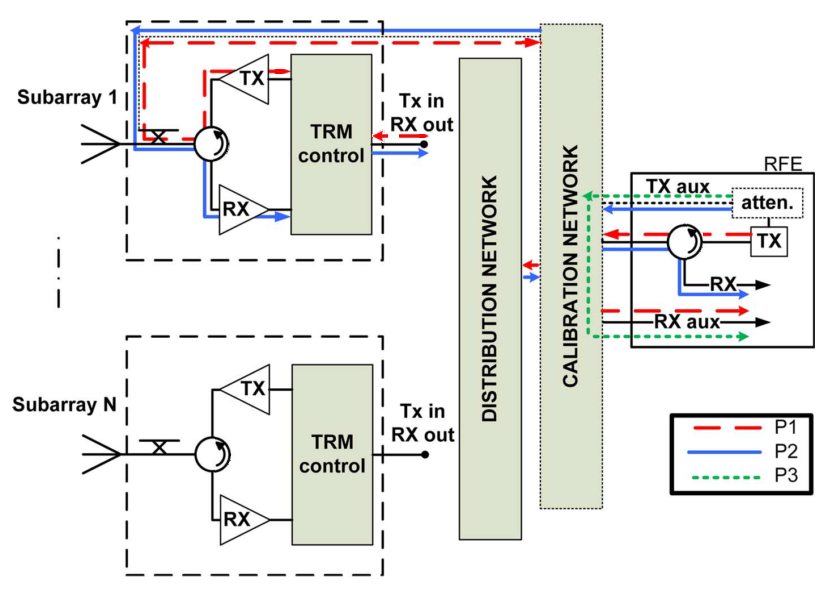
\includegraphics[width=10cm]{gfx/classic_cal_scheme.png}
 \caption{Esquema de calibración interna: camino de calibración de pulsos \textbf{P1} (Tx) en línea punteada, \textbf{P2} (Rx)
 en línea llena y \textbf{P3} (UCC) en verde \cite{Makhoul2012}.}
 \label{fig:classic_cal_scheme}
\end{figure}

Como ejemplos de sistemas que utilizaron dicho método, se puede nombrar al instrumento radar de los satélites E-ERS-1, SIR-C
\cite{Curlander1991}, terraSAR-X \cite{Schwerdt2005} y ENVISAT ASAR \cite{Loop}. La figura \ref{fig:calibrMethods} muestra los esquemas
de calibración de los primeros dos sistemas mencionados.

\begin{figure}[H]
	\centering
	\subfloat[instrumento radar del satélite E-ERS-1]{
		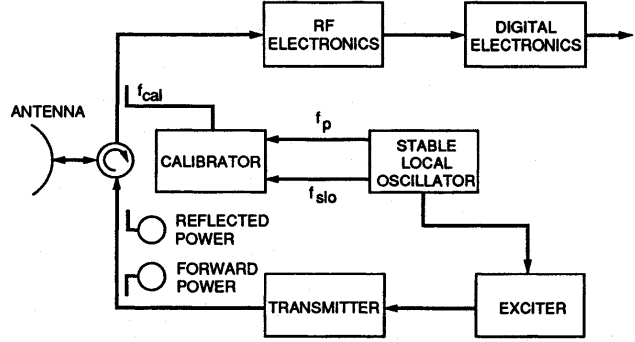
\includegraphics[width=7cm]{gfx/sirCalibration.png}}
 	\subfloat[instrumento radar del satélite SIR-C]{
		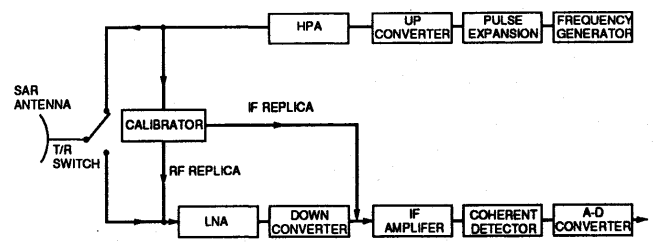
\includegraphics[width=7cm]{gfx/eersCalibration.png}}
	\caption{Esquemas de calibración interna del instrumento radar \cite{Curlander1991}.}
	\label{fig:calibrMethods}
\end{figure}


\subsection{Método} \label{ssc:classicalMethod}

No solo es necesaria la medición de la estabilidad del instrumento, sino que también se requiere obtener información del
comportamiento de los TRMs de forma individual, dado que el apuntamiento y la planitud del frente de onda de la señal dependen
de la ganancia y fase configurada de estos componentes. Por lo tanto, es necesario conocer el estado actual de los TRMs,
especialmente si se considera una posible degradación en el desempeño o mal funcionamiento de los mismos \cite{Br2007}.

Una estrategia para mediciones individuales de cada TRM requiere que el resto de dichos componentes estén apagados 
\cite{Br2007}. El problema de esta estrategia es que, al tener parte de la antena apagada, no resulta un método representativo
al modo de funcionamiento nominal (toda la antena operativa).

Para resolver este problema y calibrar todos los TRMs en simultáneo, al menos en transmisión o en recepción, se emiten
subsecuentes pulsos de calibración modificando los parámetros configurables que introducen los actuadores al sistema, en este
caso la fase introducida por los TRMs. De esta forma, se arma una codificación diferente para cada lazo de calibración de forma
tal que los distintos códigos sean ortogonales entre sí. Este algoritmo se llama PCC.

En esta tesis se utilizan los códigos walsh para codificar cada lazo de calibración \cite{WalshCode}. En esta estrategia se
configura el desfasaje de cada TRM en para cada pulso de calibración en $\pm90^{\circ}$ con respecto a la fase que poseía la
antena en el momento de iniciar el proceso de calibración. Siguiendo una determinada secuencia $c_{mn}(t)$.

\begin{figure}
 \centering
 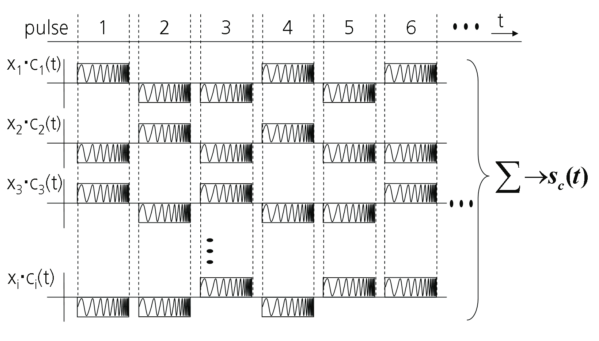
\includegraphics[width=8cm]{gfx/superposition_signals_classic.png}
 \caption{Superposición de señales de todos los TRMs. Cada señal tiene su propia secuencia de código aplicada entre pulsos
 \cite{Br2007}.}
 \label{fig:sup_sign_classic}
\end{figure}

La figura \ref{fig:sup_sign_classic} muestra la superposición de la señal de calibración con las distintas fases que adoptan
los $j$ TRMs de la antena en los $n$ pulsos requeridos para completar la codificacion utilizada.

Por lo tanto, la fase de salida de cada TRM es la fase de la señal sumada a la configurada previamente a iniciar la
calibración, $\varphi_{mn}$, junto al desfase del código de $90^{\circ}$. Consecuentemente, la superposición de todas las
ganancias de los TRMs, $a_{mn}$, y fases, $\varphi_{mn}$, es obtenida en el puerto de recepción de la RFDN, $s_c(t)$ como se
muestra en la figura \ref{fig:sup_sign_classic}.

\begin{equation}
	s_c(t) = \sum_{m=0}^{M-1}\sum_{n=0}^{N-1}c_{mn}\cdot a_{mn}e^{j\varphi{mn}} + n_{mn}
\end{equation}

Donde $n_{mn}$ es el ruido inherente que hay en las mediciones de cada TRM. Para decodificar y obtener la ganancia
$\tilde{a}_{mn}$ y fase estimada $\tilde\varphi_{mn}$ de algún TRM, la señal compuesta $s_c$ es correlacionada con
la secuencia del módulo deseado. Con esta correlación, la modulación de la secuencia se elimina dando como resultado
la ganancia estimada.

\begin{equation}
\begin{aligned}
	\tilde{x}_{mn} &= s_c \otimes c^*_{mn} \\
	\tilde{x}_{mn} = \int s_c(t) &\cdot c^*_{mn}(t) dt = \tilde{a}_{mn}e^{j\tilde{\varphi}_{mn}} \\
\end{aligned}
\label{eq:classic_correlation}
\end{equation}

En general el código de calibración utilizado es el código walsh \cite{WalshCode}. Dicho código deriva de las matrices de 
Hadamard (ver apéndice \ref{AppendixB}); dada sus propiedades de ortogonalidad, cada código, o fila, es unívocamente 
distinguible del resto. Para minimizar la cantidad de mediciones, el largo del código ($l$) debe ser lo más corto posible. 
El número de TRMs de la antena es el determinante de la cota inferior.

\begin{equation}
	l = 2^i \ge N \cdot M
\end{equation}

Asumiendo $N$ la cantidad de filas y $M$ la cantidad de paneles, o columnas, que tiene el conjunto de antena, se utilizan tres
estrategias con este método de calibración para obtener distintos niveles de granularidad de mediciones a saber.

\begin{itemize}
	\item \textbf{Nivel módulo:} Este nivel es el que utiliza los códigos más largos, dado que se calibran todos los módulos que
		posee la antena en una polarización determinada ($l = 2^i \ge N \cdot M$).
	\item \textbf{Nivel panel:} En este nivel se utiliza el mismo código para todos los TRMs que son de un mismo panel,
		logrando así, decrecer el largo del código ($l = 2^i \ge M$).
	\item \textbf{Nivel fila:} En este nivel se utiliza el mismo código para todos los TRMs que son de una misma fila,
		logrando así, decrecer el largo del código ($l = 2^i \ge N$).
\end{itemize}

Este método a nivel panel y fila sirve para la caracterización del la configuración del apuntamiento de antena \cite{Br2007}.


\subsection{Limitaciones}

La calibración clásica se utiliza típicamente con el objeto de poder detectar componentes que funcionan mal, en particular los
TRM. Puesto que si un TRM presenta alguna falla en su funcionamiento como ser por ejemplo un amplificador que no responde, esto
se puede detectar en la calibración interna clásica mediante el lazo de calibración. Sin embargo, este esquema presenta las
siguientes desventajas: 


\subsubsection{Caracterización previa de los elementos de antena}

Para poder conocer la ganancia del lazo de transmisión o recepción es necesario conocer la potencia de la señal de
calibración, para sustraerla del resultado obtenido. El lazo de calibración donde se realiza esta medición es el que se
muestra en la imagen \ref{fig:classic_cal_scheme}, llamado \textbf{P3}. En esta medición no se puede determinar cuanto atenúa
el lazo, por lo tanto se opta por caracterizar en tierra dichos componentes para las frecuencias y temperaturas de trabajo.

Tener que recurrir a las caracterizaciones a los componetnes de la antena presentan las siguientes desventajas: 

\begin{itemize}
	\item Costo de materiales: Componentes caracterizados en temperatura pueden costar varias veces el precio de un componente sin
		caracterizar. Esto es debido a que los ensayos de caracterización térmicos son costosos. Tambien lo es el equipamiento para
		realizar las características en frecuencia y muchas veces son rentados por las compañias ante la imposibilidad de comprarlos.
	\item Costo de recursos: La campaña de caracterización no solo puede durar meses sino que también requiere una dedicación
		casi total de equipos de gente a dicha actividad, implicando un gasto de dinero muy importante. En algunos proyectos donde hay
		fechas preacordadas que respetar, pueden determinar que dichos costos sean inviables.
	\item Comportamiento de materiales fin de vida: Como el material envejece, cambia sus propiedades, por lo tanto las mediciones
		realizadas en la campaña de caracterización dejan de tener validez.
\end{itemize}


\subsubsection{Complejidad del hardware de la antena}

Como se calibra sólo una parte de la antena por vez, transmisión o recepción en una u otra polarización (H o V), es necesario
que el lazo de calibración esté compuesto por la parte de la antena a calibrar junto a hardware dedicado (cables y switches) a
esta tarea. De esta forma, se añaden las siguientes desventajas:

\begin{itemize}
	\item Incremento en complejidad de HW: El HW de la antena resulta más complejo por el agregado de componentes dedicados a la
		calibración.
	\item Caracterizaciones extra: Se debe caracterizar el HW dedicado a la calibración, para restar el desfase y atenuación
		agregado en el momento de realizar la calibración.
	\item Acoplamiento: Como hay hardware agregado, es debe tomar recaudo ante el incremento de los posibles acoplamientos entre
		componentes.	
\end{itemize}


\subsubsection{Susceptibilidad ante inestabilidad del generador}

Este método es susceptible a las variaciones de fase y potencia del generador entre pulsos de calibración. Por lo tanto, es de
vital importancia contar con un generador que sea estable.


\subsubsection{Sistema incompleto}

Como hay componentes que están fuera de los lazos de calibración, con el método nunca se puede determinar de forma totalmente
correcta la ganancia de la antena en cualquiera de sus modos.


\subsubsection{Optimización en la longitud de código del PCC}

A la hora de elegir la longitud del código Walsh, es importante que siempre haya un elemento radiante virtual en la antena para
evitar la primer columna de la matriz de códigos. En caso contrario el primer TRM siempre tendrá un error en la estimación de
su ganancia \cite{Wang2010}.


\subsubsection{Pérdida de ortogonalidad en el código utilizado por comportamiento de desfasadores}

Si el desfasador no tiene un comportamiento exactamente igual al configurado a la hora de realizar la calibración, los códigos
walsh pierden ortogonalidad y, por ende, se logra obtener una mala estimación de los valores de ganancia de la antena.


\subsubsection{Compensación de temperatura en elementos}

Se debe mantener la temperatura de los elementos en los valores caracterizados para garantizar que las calibraciones sirven.


\subsubsection{Dependencia del modelo y análisis térmico}

Es completamente dependiente del modelo y análisis térmico. Por ejemplo, se asume que el comportamiento de los elementos
radiantes de la antena no varían con la temperatura.

\section{Conclusiones}

En este capítulo se introdujo tanto el modelo matemático de la calibración interna clásica como su forma de operar. A su vez,
se brindaron ejemplos de satélites en donde su sistema de radar utiliza este método.

Por último, se llegó a la conclusión que este método sirve para poder determinar que un TRM funcione correctamente, pero si
se lo desea utilizar con otro objetivo, por ejemplo el de corregir la planitud de la señal transmitida, hay que tener recaudos
en la cantidad de inconvenientes que trae aparejado. Por ejemplo, los costos en tiempo y recursos asociados a la campaña de 
caracterización y que se tenga fe de que con el envejecimiento de los componentes, dichas caracterizaciones van a continuar
sirviendo.

